\section{技術検証}
作成したシステムの動作検証を行った。

\subsection{検証シナリオ}
技術検証は,1台のIoT機器で成り立っているIoTサービスを想定し行った.
IoT機器には,RaspberryPiを使用する.
図\ref{fig:device}は使用したRaspberryPi2と,IntelEdisonである.
今回は、IntelEdisonは使用していないが,参考の為に上げた.
%IoT機器の図
\begin{figure}[htbp]
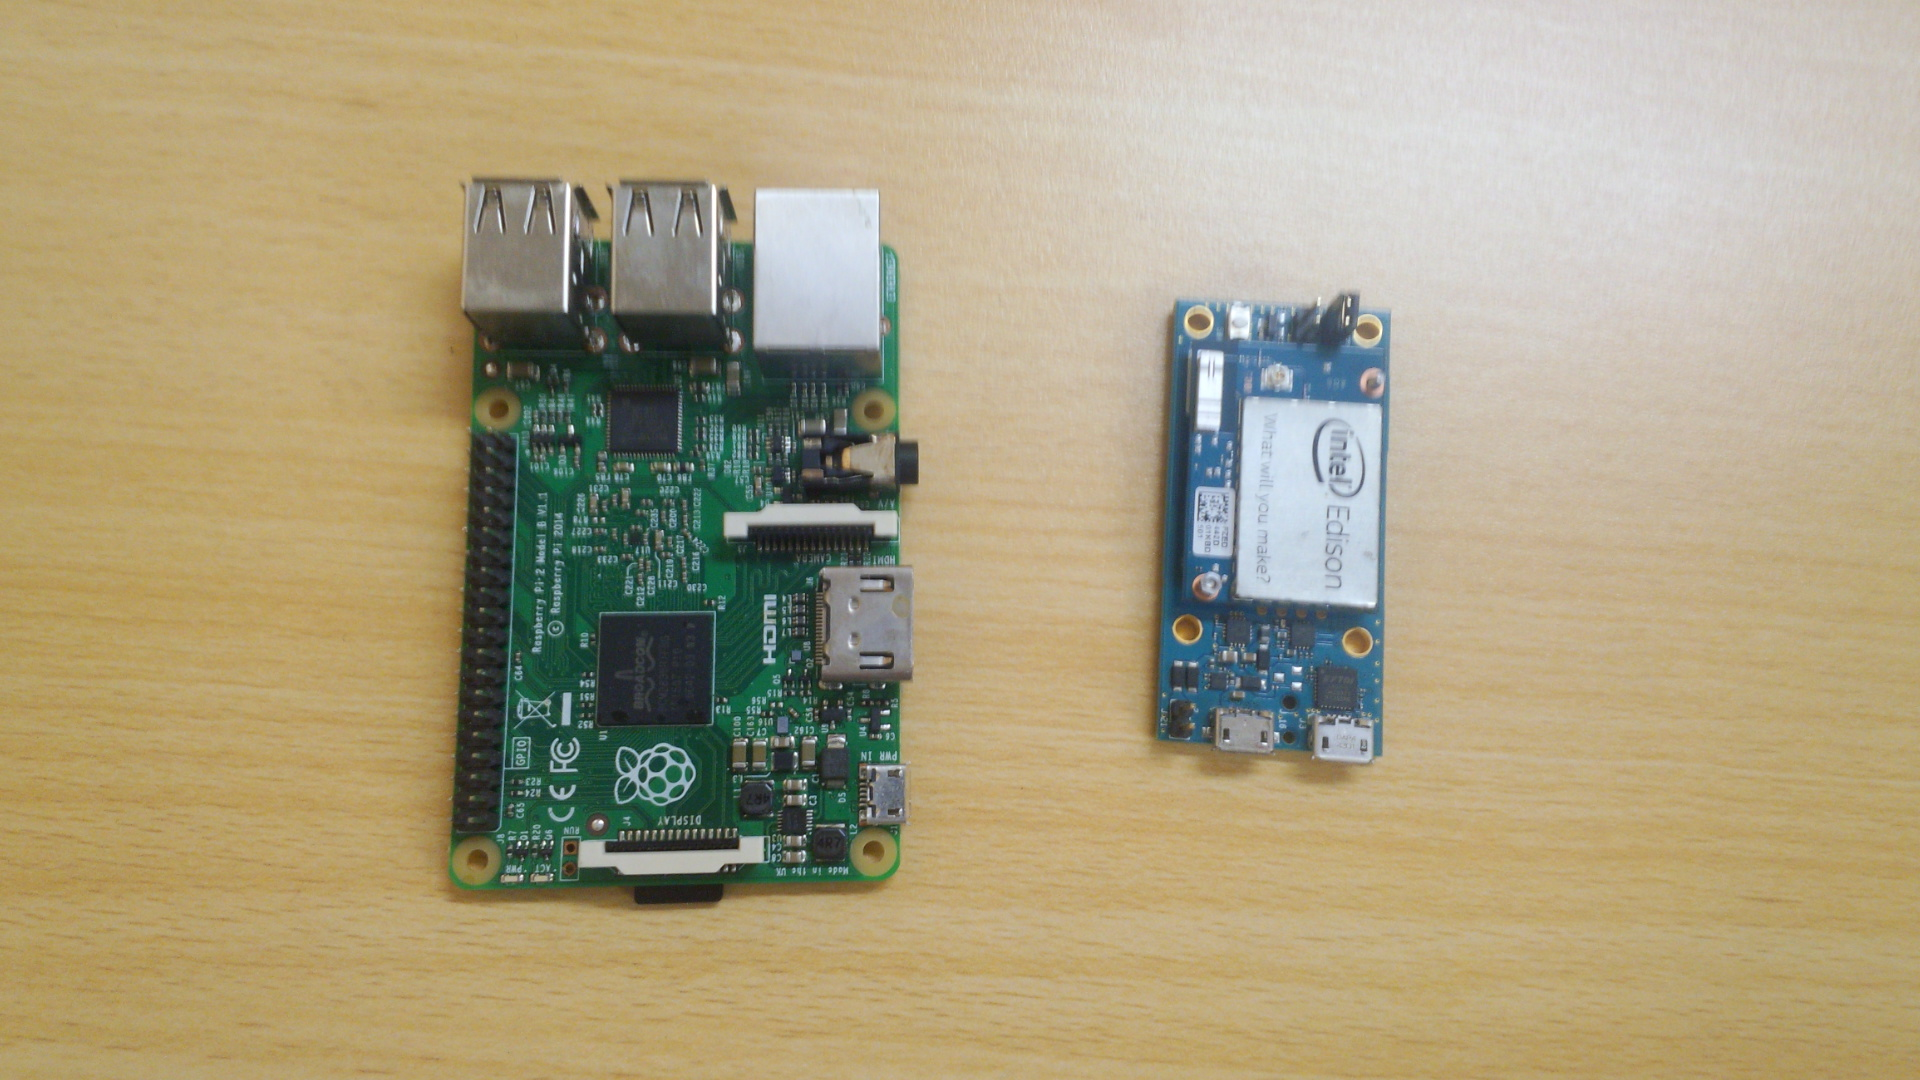
\includegraphics[width=14cm]{images/device.png}
\caption{IoTサービスの構成図}
\label{fig:device}
\end{figure}

RaspberyPi2は無線LANインターフェースを持たないので,バファロー製の無線LANインターフェースを使用した.

期間は2017年1月28日正午から1時間行い,途中何度かIoT機器(RaspberryPi)の電源を抜き,正常に検知することを確認する.
その後,電源が抜けていた期間について,IoT機器の記録を確認する.

\subsection{検証結果}
IoT機器の監視については問題なく動作した事を確認した.
機器の電源を抜くと、1分程度で表示状態が変わり、
数分後、機器の電源を再び入れると、2分程度で表示状態が戻ることを確認した.


\begin{enumerate}
\item 予め固有のIDとエージェントプログラムがインストールされた機器を買ってくる
\item ユーザは、その機器に対しサービスで利用するアプリケーションをインストールし、設置する
\item 機器は、設置後ネットワークに接続され次第、サービスへ、機器の状態の通知を行う
\end{enumerate}
IoTサービス提供者が手軽に利用できることを確認した。


\section{サービスの特徴}
他の関し手法と比較した本サービスの特徴として、通知型で設定不要、規模に対応できることが挙げられる。
独立したサービスとしてまとまっていることが挙げられる。




\section{考察}
ユーザーテストから本システムは,ある程度有効であることが分かったが,以下の点について課題があることが分かった.
\begin{itemize}
\item 機器への設定について\\
	設定ファイルの編集等の手間は削減されたが,エージェントプログラムをIoT機器にインストールするのに手間がかかっていることが分かった.
	従来手法を用いて機器の監視をする際は,自動起動の設定を行う必要はなかったが,本プログラムでは必要としている.
	自動起動の為の設定ファイルを自動生成するか,あるいはエージェントプログラム配布の際,簡単なインストールスクリプト等を一緒に配布することで,大きな手間の削減になると感じでいる.
\item ユーザーインターフェースについて\\
	現在,過去の機器状態の記録については,文字記録として表示しているが,グラフ表示等の方が見やすいと感じた.
	また,期間を指定して閲覧できる機能も必要であることが分かった.
\item エージェントプログラムについて\\
	本サービスで提供しているエージェントプログラムは,その他のパッケージに依存しない単純な構成であるため,移植性が高い.
\end{itemize}
また、本来ならば、株式会社ルナネクサスにて、使用して頂き、評価を得る必要があったが、双方のスケジュールの都合と開発の遅れから行うことが出来なかった。
しかし、今後IoTサービスの開発が盛んになることや、使用するIoT機器の数が多くなることから、本サービスの必要性は高くなっていくと考えられる。


